\documentclass{standalone}
\usepackage{tikz}
\usetikzlibrary{patterns, positioning}
\usepackage[sfdefault]{ClearSans} %% option 'sfdefault' activates Clear Sans as the default text font
\usepackage[T1]{fontenc}

\begin{document}
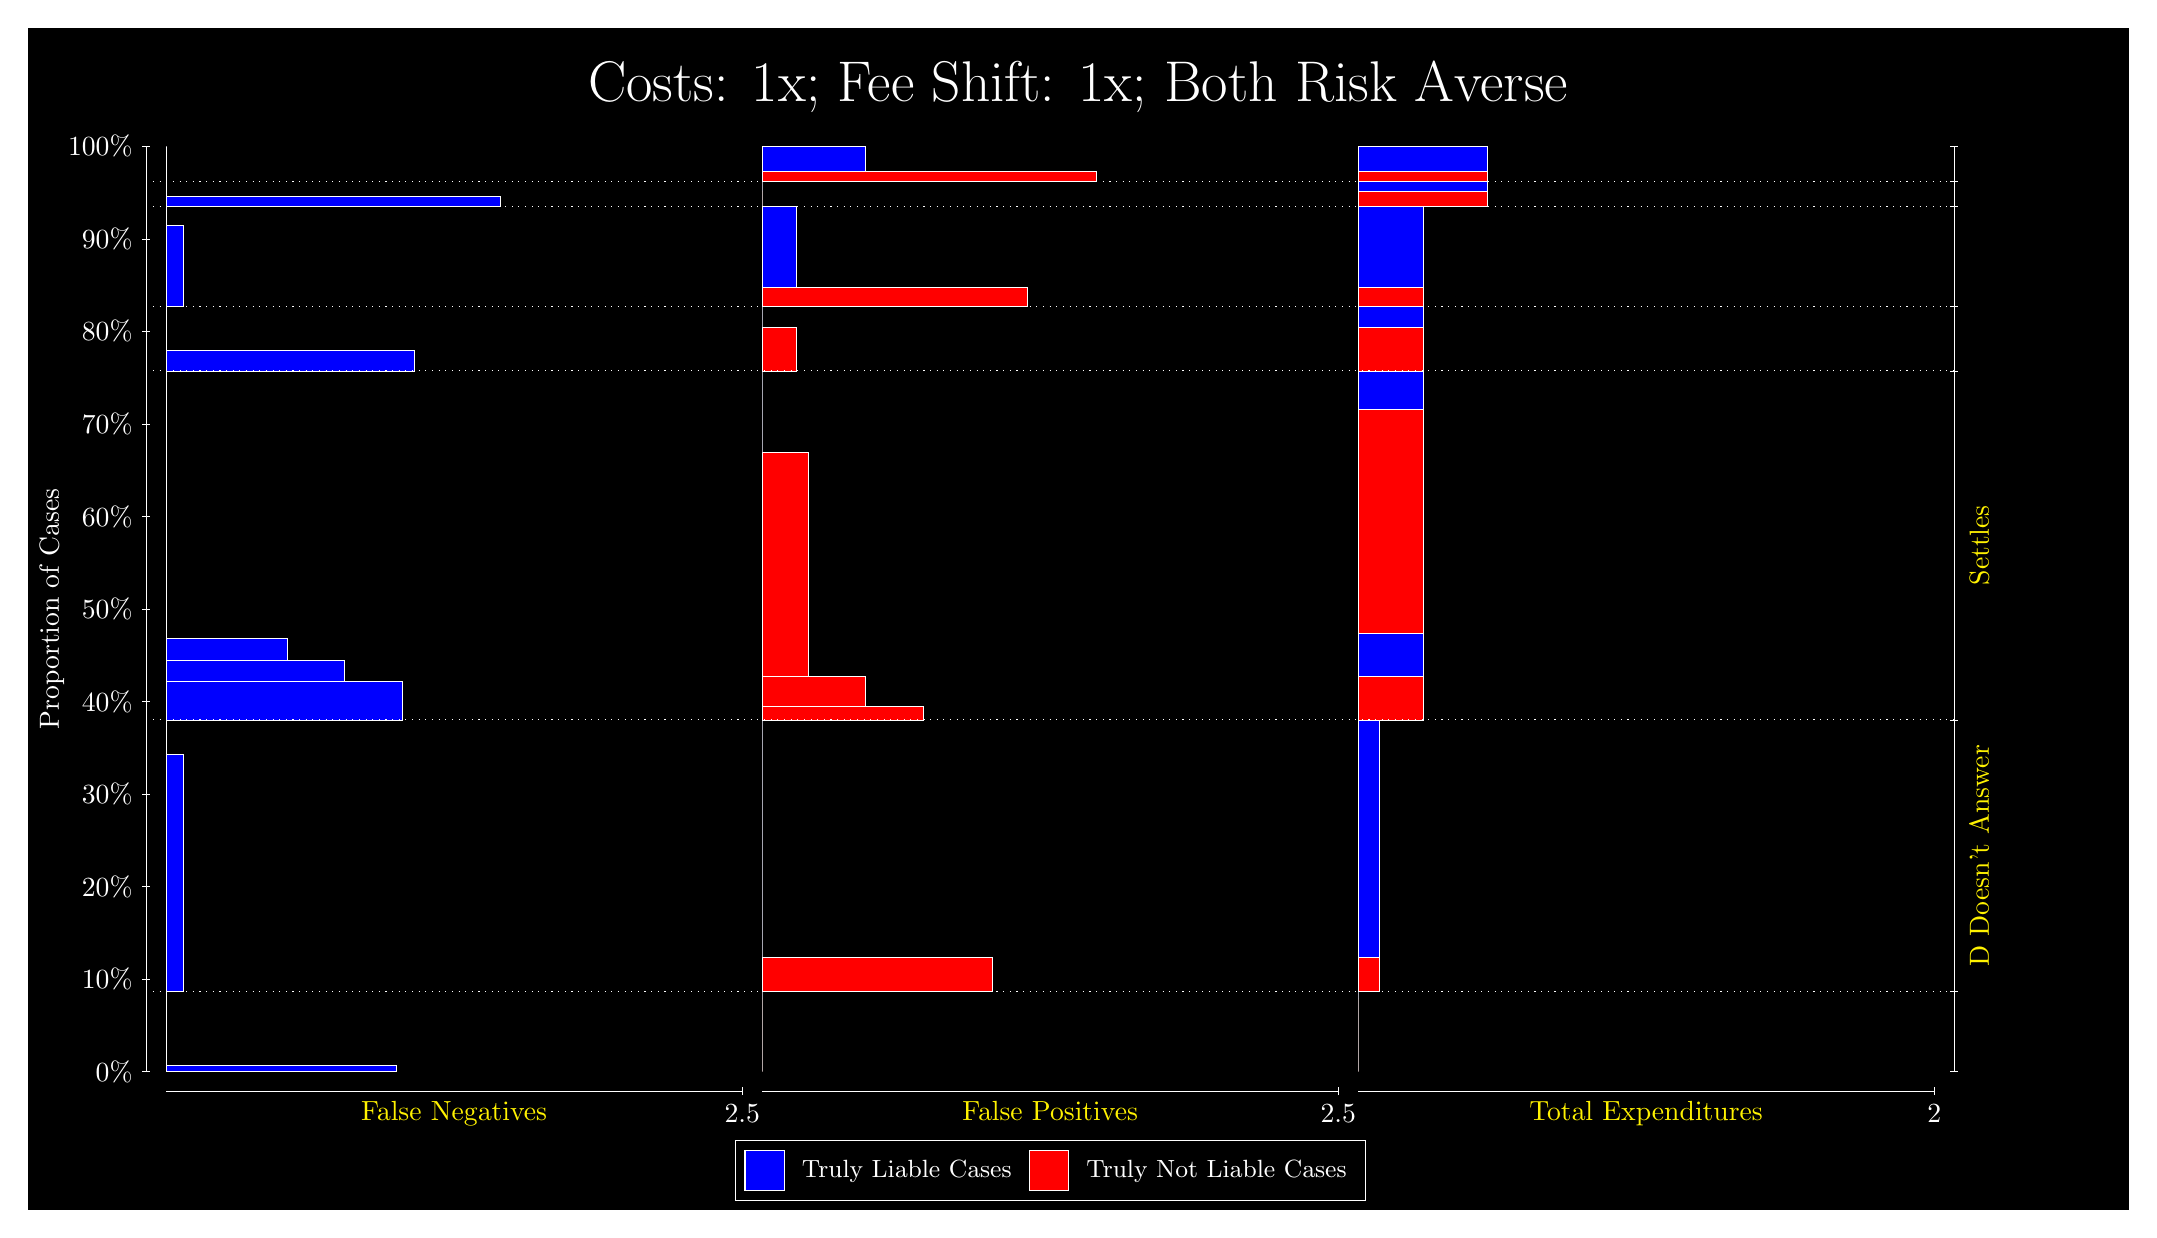
\begin{tikzpicture}
\draw[fill=black] (0,0) rectangle (26.667,15);
\draw[text=white] (0,13.5) rectangle (26.667,15) node[midway] {\huge Costs: 1x; Fee Shift: 1x; Both Risk Averse};
\draw[white, very thin] (1.5,1.75) -- (1.5,13.5);
\node[rotate=90, text=white, anchor=center] at (0.3, 7.625) {Proportion of Cases};
\draw[white, very thin] (1.45,1.75) -- (1.55,1.75);
\node[text=white, anchor=east] at (1.45, 1.75) {0\%};
\draw[white, very thin] (1.45,2.925) -- (1.55,2.925);
\node[text=white, anchor=east] at (1.45, 2.925) {10\%};
\draw[white, very thin] (1.45,4.1) -- (1.55,4.1);
\node[text=white, anchor=east] at (1.45, 4.1) {20\%};
\draw[white, very thin] (1.45,5.275) -- (1.55,5.275);
\node[text=white, anchor=east] at (1.45, 5.275) {30\%};
\draw[white, very thin] (1.45,6.45) -- (1.55,6.45);
\node[text=white, anchor=east] at (1.45, 6.45) {40\%};
\draw[white, very thin] (1.45,7.625) -- (1.55,7.625);
\node[text=white, anchor=east] at (1.45, 7.625) {50\%};
\draw[white, very thin] (1.45,8.8) -- (1.55,8.8);
\node[text=white, anchor=east] at (1.45, 8.8) {60\%};
\draw[white, very thin] (1.45,9.975) -- (1.55,9.975);
\node[text=white, anchor=east] at (1.45, 9.975) {70\%};
\draw[white, very thin] (1.45,11.15) -- (1.55,11.15);
\node[text=white, anchor=east] at (1.45, 11.15) {80\%};
\draw[white, very thin] (1.45,12.325) -- (1.55,12.325);
\node[text=white, anchor=east] at (1.45, 12.325) {90\%};
\draw[white, very thin] (1.45,13.5) -- (1.55,13.5);
\node[text=white, anchor=east] at (1.45, 13.5) {100\%};

\draw[white, very thin] (24.457,1.75) -- (24.457,13.5);
\draw[white, very thin] (24.407,1.75) -- (24.507,1.75);
\node[anchor=west] at (24.407, 1.75) {};
\draw[white, very thin] (24.407,2.7636) -- (24.507,2.7636);
\node[anchor=west] at (24.407, 2.7636) {};
\draw[white, very thin] (24.407,6.2171) -- (24.507,6.2171);
\node[anchor=west] at (24.407, 6.2171) {};
\draw[white, very thin] (24.407,10.649) -- (24.507,10.649);
\node[anchor=west] at (24.407, 10.649) {};
\draw[white, very thin] (24.407,11.468) -- (24.507,11.468);
\node[anchor=west] at (24.407, 11.468) {};
\draw[white, very thin] (24.407,12.739) -- (24.507,12.739);
\node[anchor=west] at (24.407, 12.739) {};
\draw[white, very thin] (24.407,13.058) -- (24.507,13.058);
\node[anchor=west] at (24.407, 13.058) {};
\draw[white, very thin] (24.407,13.5) -- (24.507,13.5);
\node[anchor=west] at (24.407, 13.5) {};

\draw[white, very thin, fill=blue] (1.75,1.75) rectangle (4.6775,1.832);
\draw[white, very thin, fill=red] (1.75,1.832) rectangle (1.75,2.7636);
\draw[white, very thin, fill=blue] (1.75,2.7636) rectangle (1.9696,5.7792);
\draw[white, very thin, fill=red] (1.75,5.7792) rectangle (1.75,6.2171);
\draw[white, very thin, fill=blue] (1.75,6.2171) rectangle (4.7507,6.7097);
\draw[white, very thin, fill=blue] (1.75,6.7097) rectangle (4.0188,6.9713);
\draw[white, very thin, fill=blue] (1.75,6.9713) rectangle (3.287,7.2562);
\draw[white, very thin, fill=red] (1.75,7.2562) rectangle (1.75,10.649);
\draw[white, very thin, fill=blue] (1.75,10.649) rectangle (4.8971,10.916);
\draw[white, very thin, fill=red] (1.75,10.916) rectangle (1.75,11.468);
\draw[white, very thin, fill=blue] (1.75,11.468) rectangle (1.9696,12.497);
\draw[white, very thin, fill=red] (1.75,12.497) rectangle (1.75,12.739);
\draw[white, very thin, fill=blue] (1.75,12.739) rectangle (5.9949,12.867);
\draw[white, very thin, fill=red] (1.75,12.867) rectangle (1.75,13.058);
\draw[white, very thin, fill=red] (1.75,13.058) rectangle (1.75,13.186);
\draw[white, very thin, fill=blue] (1.75,13.186) rectangle (1.75,13.5);
\draw[white, very thin, fill=red] (9.3189,1.75) rectangle (9.3189,2.6815);
\draw[white, very thin, fill=blue] (9.3189,2.6815) rectangle (9.3189,2.7636);
\draw[white, very thin, fill=red] (9.3189,2.7636) rectangle (12.246,3.2015);
\draw[white, very thin, fill=blue] (9.3189,3.2015) rectangle (9.3189,6.2171);
\draw[white, very thin, fill=red] (9.3189,6.2171) rectangle (11.368,6.3949);
\draw[white, very thin, fill=red] (9.3189,6.3949) rectangle (10.636,6.7718);
\draw[white, very thin, fill=red] (9.3189,6.7718) rectangle (9.9044,9.6099);
\draw[white, very thin, fill=blue] (9.3189,9.6099) rectangle (9.3189,10.649);
\draw[white, very thin, fill=red] (9.3189,10.649) rectangle (9.758,11.201);
\draw[white, very thin, fill=blue] (9.3189,11.201) rectangle (9.3189,11.468);
\draw[white, very thin, fill=red] (9.3189,11.468) rectangle (12.686,11.71);
\draw[white, very thin, fill=blue] (9.3189,11.71) rectangle (9.758,12.739);
\draw[white, very thin, fill=red] (9.3189,12.739) rectangle (9.3189,12.93);
\draw[white, very thin, fill=blue] (9.3189,12.93) rectangle (9.3189,13.058);
\draw[white, very thin, fill=red] (9.3189,13.058) rectangle (13.564,13.186);
\draw[white, very thin, fill=blue] (9.3189,13.186) rectangle (10.636,13.5);
\draw[white, very thin, fill=red] (16.888,1.75) rectangle (16.888,2.6815);
\draw[white, very thin, fill=blue] (16.888,2.6815) rectangle (16.888,2.7636);
\draw[white, very thin, fill=red] (16.888,2.7636) rectangle (17.162,3.2015);
\draw[white, very thin, fill=blue] (16.888,3.2015) rectangle (17.162,6.2171);
\draw[white, very thin, fill=red] (16.888,6.2171) rectangle (17.711,6.7718);
\draw[white, very thin, fill=blue] (16.888,6.7718) rectangle (17.711,7.3184);
\draw[white, very thin, fill=red] (16.888,7.3184) rectangle (17.711,10.156);
\draw[white, very thin, fill=blue] (16.888,10.156) rectangle (17.711,10.649);
\draw[white, very thin, fill=red] (16.888,10.649) rectangle (17.711,11.201);
\draw[white, very thin, fill=blue] (16.888,11.201) rectangle (17.711,11.468);
\draw[white, very thin, fill=red] (16.888,11.468) rectangle (17.711,11.71);
\draw[white, very thin, fill=blue] (16.888,11.71) rectangle (17.711,12.739);
\draw[white, very thin, fill=red] (16.888,12.739) rectangle (18.534,12.93);
\draw[white, very thin, fill=blue] (16.888,12.93) rectangle (18.534,13.058);
\draw[white, very thin, fill=red] (16.888,13.058) rectangle (18.534,13.186);
\draw[white, very thin, fill=blue] (16.888,13.186) rectangle (18.534,13.5);
\draw[white, dotted] (1.5,2.7636) -- (24.457,2.7636);
\draw[white, dotted] (1.5,6.2171) -- (24.457,6.2171);
\draw[white, dotted] (1.5,10.649) -- (24.457,10.649);
\draw[white, dotted] (1.5,11.468) -- (24.457,11.468);
\draw[white, dotted] (1.5,12.739) -- (24.457,12.739);
\draw[white, dotted] (1.5,13.058) -- (24.457,13.058);
\draw[white, very thin] (1.75,1.5) -- (9.0689,1.5);
\node[text=yellow, anchor=north] at (5.4094, 1.5) {False Negatives};
\draw[white, very thin] (9.0689,1.45) -- (9.0689,1.55);
\node[text=white, anchor=north] at (9.0689, 1.45) {2.5};

\draw[white, very thin] (9.3189,1.5) -- (16.638,1.5);
\node[text=yellow, anchor=north] at (12.978, 1.5) {False Positives};
\draw[white, very thin] (16.638,1.45) -- (16.638,1.55);
\node[text=white, anchor=north] at (16.638, 1.45) {2.5};

\draw[white, very thin] (16.888,1.5) -- (24.207,1.5);
\node[text=yellow, anchor=north] at (20.547, 1.5) {Total Expenditures};
\draw[white, very thin] (24.207,1.45) -- (24.207,1.55);
\node[text=white, anchor=north] at (24.207, 1.45) {2};


\node[text=yellow, centered, rotate=90] at (24.777, 4.4903) {D Doesn't Answer};
\node[text=yellow, centered, rotate=90] at (24.777, 8.4331) {Settles};





\draw (12.978300999999998,1.5) node[draw=none] (baseCoordinate) {};
\begin{scope}[align=center]
        \matrix[scale=0.5, draw=white, below=0.5cm of baseCoordinate, nodes={draw}, column sep=0.1cm]{
            \node[rectangle, draw, minimum width=0.5cm, minimum height=0.5cm, fill=blue] {}; &
            \node[draw=none, font=\small, text=white] (B) {Truly Liable Cases}; &
            \node[rectangle, draw, minimum width=0.5cm, minimum height=0.5cm, fill=red] {}; &
            \node[draw=none, font=\small, text=white] (B) {Truly Not Liable Cases}; \\
            };
\end{scope}

\end{tikzpicture}
\end{document}